\documentclass[11pt]{article}
\usepackage[margin=0.9in]{geometry}
\usepackage[T1]{fontenc}
\usepackage{lmodern,amsmath,amssymb,bm,graphicx,booktabs,microtype,hyperref,placeins}
\hypersetup{colorlinks=true,urlcolor=blue,citecolor=blue,linkcolor=blue}
\newcommand{\dd}{\mathrm d}
\newcommand{\D}{D_{\!L}}
\newcommand{\tb}{t_{\rm B}}
\title{Bang-time perturbations and redshift drift in a parabolic LTB model:\\ a reproducible light-cone calculation}
\author{Dani Postma (DXN1)\\\small Independent researcher}
\date{17 October 2026\\\small Preprint, version 1.1}
\begin{document}
\maketitle
\begin{abstract}
We calculate the response of redshift drift to a radially varying bang time in an exactly solvable, parabolic Lema\^itre--Tolman--Bondi (LTB) dust spacetime. The drift is propagated between neighboring light cones rather than inferred from a Friedmann--Lema\^itre--Robertson--Walker (FLRW) endpoint formula. We derive an explicit variational system and compare its response with finite differences. Two smooth, centrally regular bang-time perturbations yield negative equal-luminosity-distance responses at all 15 sampled baseline redshifts $0.1\leq z\leq1.5$; no zero crossing appears in these examples. We quantify how equal-distance and fixed-redshift comparisons differ, and how the FLRW endpoint shortcut misestimates the response. This dimensionless dust example is neither an observational fit nor a uniqueness result. We identify the functional distance compensation, background realism, and physical constraints needed for a cosmological inference.
\end{abstract}

\section{Scope and relation to earlier work}
Redshift drift in spherically symmetric spacetimes and its use with distance data were established by Uzan, Clarkson and Ellis~\cite{uzan}. Yoo, Kai and Nakao developed the LTB drift calculation and studied void models~\cite{yoo}. Exact growing and decaying density modes in LTB dust have been analyzed by Sussman~\cite{sussman}. The inverse problem for LTB observables has additional existence and regularity conditions~\cite{inverse}. We therefore claim neither a new general drift equation nor a unique observational signature. The purpose here is to correct an endpoint-formula error in an earlier unpublished draft, spell out an explicit parameter derivative, and give a small reproducible test case.

In units $c=G=1$, the LTB metric and evolution equation are
\begin{align}
\dd s^2&=-\dd t^2+\frac{R'(t,r)^2}{1+2E(r)}\dd r^2+R(t,r)^2\dd\Omega^2,\label{eq:metric}\\
\dot R^2&=\frac{2M(r)}{R}+2E(r),\qquad R(\tb(r),r)=0.\label{eq:field}
\end{align}
Dots and primes denote partial derivatives at fixed $r$ and $t$, respectively. A radial coordinate choice removes one of $M,E,\tb$ as an independent function. A nonconstant $\tb$ represents the decaying mode in the conventional LTB dust mode decomposition~\cite{sussman}; its additive constant sets the time origin. Throughout this paper the mass-coordinate gauge and the profiles below are specified explicitly.

The calculation is organized around five questions. (i) What is the drift of the \emph{same comoving source} when the central observer's clock advances? (ii) Does a bang-time perturbation give the same derivative at fixed redshift and at equal luminosity distance? (iii) Does either of the specified perturbations force a zero crossing? (iv) How large is the error from importing the FLRW endpoint expression into LTB? (v) What further constraints are required before a response can be identified as an observable decaying-mode signal? Equations~\eqref{eq:ray}--\eqref{eq:fixedD} answer the first two mathematically; Secs.~4--6 test the middle questions and delimit the last one.

\section{Drift on neighboring radial light cones}
Put $S(r)=\sqrt{1+2E(r)}$, $A=R'/S$, $B=\dot R'/S$, and $C=\ddot R'/S$. On an incoming radial ray from a central, comoving observer at $r=0$, the emission time $t(r)$ and observed redshift $z(r)$ satisfy
\begin{equation}
\frac{\dd t}{\dd r}=-A,\qquad \frac{\dd z}{\dd r}=(1+z)B,\qquad t(0)=t_0,\quad z(0)=0.\label{eq:ray}
\end{equation}
Compare two rays received at times separated by $\delta t_0$, from the \emph{same comoving emitter} $r$. Their time separation $T(r)=\partial t(r;t_0)/\partial t_0$ obeys $T'=-BT$, $T(0)=1$, hence $T=1/(1+z)$. Let $Z(r)=\partial z(r;t_0)/\partial t_0$ be drift per unit central proper time. Differentiating Eq.~\eqref{eq:ray} with respect to $t_0$ at fixed $r$ gives the exact propagation equation
\begin{equation}
Z'=BZ+(1+z)CT=BZ+C,\qquad Z(0)=0,\label{eq:drift}
\end{equation}
or, equivalently,
\begin{equation}
\boxed{\quad Z(r)=(1+z(r))\int_0^r\frac{C(\bar r)}{1+z(\bar r)}\,\dd\bar r.\quad}\label{eq:integral}
\end{equation}
This result carries the information along the ray. In a homogeneous FLRW limit it reduces to $Z=(1+z)H_0-H(t_e)$. In a general LTB geometry, replacing Eq.~\eqref{eq:drift} by $(1+z)H_0-\dot R'/R'|_e$ is not justified: the gradient of expansion along the ray contributes. For an isotropic central observer, reciprocity gives
\begin{equation}
\D(r)=(1+z(r))^2R(t(r),r).\label{eq:distance}
\end{equation}

\section{Linear response and what ``fixed distance'' means}
Let $p$ denote a model parameter and $\bm y=(t,z,Z)$. With $\bm y'=\bm F(\bm y,r,p)$ from Eqs.~\eqref{eq:ray} and \eqref{eq:drift}, its first-order variation $\bm u=\partial_p\bm y|_r$ is specified, without finite differences, by
\begin{equation}
\bm u'=\underbrace{\begin{pmatrix}
-A_t&0&0\\(1+z)B_t&B&0\\ B_tZ+C_t&0&B
\end{pmatrix}}_{\bm F_{\bm y}}\bm u+
\begin{pmatrix}-A_p\\(1+z)B_p\\B_pZ+C_p\end{pmatrix},\qquad \bm u(0)=\bm0.\label{eq:sensitivity}
\end{equation}
All partial derivatives in this equation are at fixed $t,r$; in particular, $A_p$ includes any parameter dependence in $S$. Equation~\eqref{eq:sensitivity} is the analytic variational equation used to define the linear response; the public numerical example evaluates its derivative by symmetric finite differences and checks step convergence.

At a given emitter coordinate the distance response is
\begin{equation}
\partial_p\D|_r=(1+z)^2(R_t t_p+R_p)+2(1+z)Rz_p,
\qquad
\frac{\dd\D}{\dd r}=2(1+z)z_rR+(1+z)^2(R_t t_r+R_r).\label{eq:Dderivs}
\end{equation}
Here $R_p$ and $R_r$ are partial derivatives, whereas $\dd\D/\dd r$ is a total derivative along the ray. If $\dd\D/\dd r\ne0$, implicit differentiation yields the response at a \emph{single equal luminosity distance},
\begin{equation}
\boxed{\left.\frac{\partial Z}{\partial p}\right|_{\D}=Z_p|_r-\frac{Z_r}{\dd\D/\dd r}\,\partial_p\D|_r.}\label{eq:fixedD}
\end{equation}
For comparison, $\partial_p Z|_z=Z_p|_r-(Z_r/z_r)z_p|_r$. Neither condition requires $\D(z)$ to be identical between the two models. Keeping the \emph{whole function} $\D(z)$ fixed would require a compensating functional perturbation in $M$ or $E$ and is a distinct inverse problem. Equations~\eqref{eq:sensitivity}--\eqref{eq:fixedD} also show that a zero-crossing location cannot be inferred from the background profile alone without specifying the allowed perturbation and compensation.

\section{Exactly specified illustrative model}
Set $t_0=1$, $E(r)=0$, $M(r)=2r^3/9$, and $\tb(r)=\epsilon f_w(r)$, with
\begin{equation}
f_w(r)=r^2\exp[-(r/w)^2],\qquad w\in\{0.8,1.2\}.\label{eq:profile}
\end{equation}
All coordinates and drift values in this section are dimensionless. The two choices of $w$ are perturbation shapes on the \emph{same homogeneous background}, not two realistic void profiles. The even behavior at $r=0$ makes the center smooth. The exact expanding solution, with $\tau=t-\epsilon f_w(r)$, is
\begin{align}
R&=r\tau^{2/3},\nonumber\\
R'&=\tau^{2/3}-\frac{2r\epsilon f'_w}{3\tau^{1/3}},\quad
\dot R'=\frac{2}{3\tau^{1/3}}+\frac{2r\epsilon f'_w}{9\tau^{4/3}},\label{eq:exact}\\
\ddot R'&=-\frac{2}{9\tau^{4/3}}-\frac{8r\epsilon f'_w}{27\tau^{7/3}}.\nonumber
\end{align}
The expansion branch requires $\tau>0$; the code checks $R'>0$ and monotonic $z,\D$ on every sampled light cone. At $\epsilon=0$, the model is Einstein--de Sitter (EdS) and has the exact check
\begin{equation}
Z_{\rm EdS}(z)=\frac23\big[(1+z)-(1+z)^{3/2}\big].\label{eq:eds}
\end{equation}
At $\epsilon\ne0$ we hold $M,E,t_0$ fixed, integrate to $z=1.6$, and compare drift values at the \emph{baseline} $\D(z)$ for $z=0.1,0.2,\ldots,1.5$. The derivative uses $[Z(+h)-Z(-h)]/(2h)$ at $h=0.002,0.001,0.0005$. The plotted result uses $h=0.0005$.

At $\epsilon=0$, the full null-cone solution provides further independent checks:
\begin{equation}
t(r)=(1-r/3)^3,\qquad 1+z(r)=(1-r/3)^{-2},\qquad
\D(z)=3\big[(1+z)-\sqrt{1+z}\big].\label{eq:edscone}
\end{equation}
The source radius corresponding to a baseline redshift is $r(z)=3[1-(1+z)^{-1/2}]$. It is this baseline distance and radius, rather than the perturbed model's redshift label, that define the equal-distance sample.

\begin{figure}[t]
\centering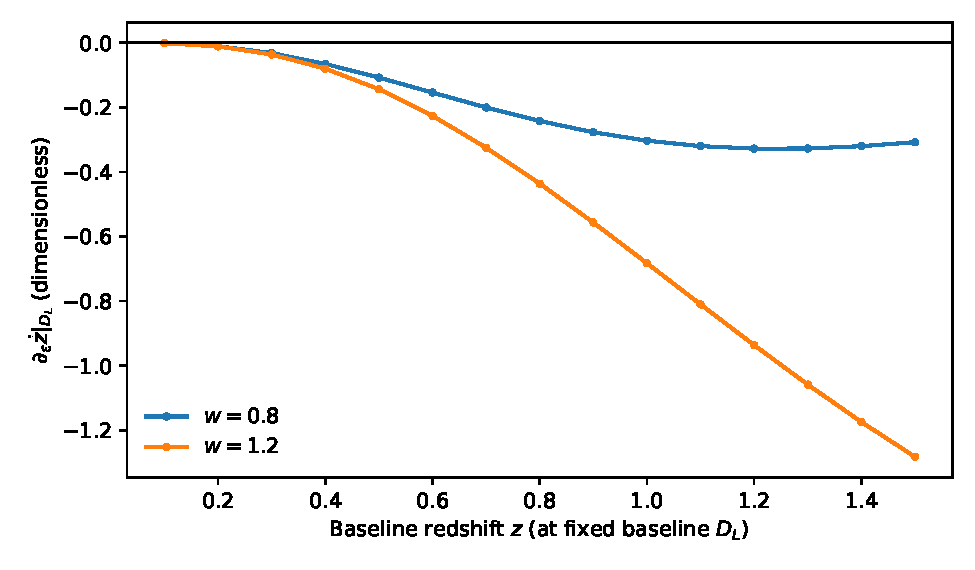
\includegraphics[width=.82\linewidth]{results/fixed_distance_response.pdf}
\caption{Dimensionless bang-time response at equal $\D$ for the two specified $f_w$. The horizontal coordinate labels the \emph{baseline} redshift. Lines guide the eye between 15 sampled points; no observational uncertainties are implied.}\label{fig:response}
\end{figure}

\begin{figure}[t]
\centering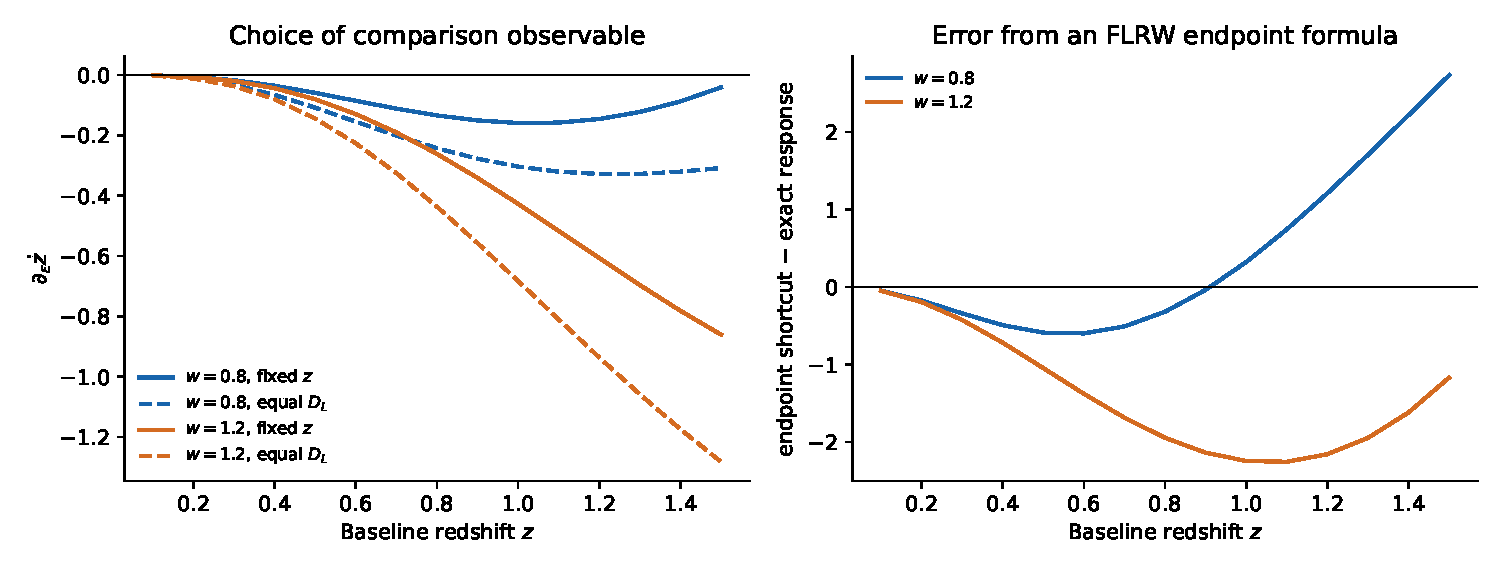
\includegraphics[width=\linewidth]{results/comparison_and_endpoint_error.pdf}
\caption{\emph{Left:} Fixed-$z$ (solid) and equal-$\D$ (dashed) derivatives for each bang-time width. \emph{Right:} Derivative from the FLRW endpoint shortcut minus the correct fixed-$z$ drift derivative. This difference can change sign with perturbation shape. Both panels use the same dimensionless parameter and baseline redshift grid.}\label{fig:comparisons}
\end{figure}

\begin{table}[t]
\centering
\caption{Diagnostics produced by \texttt{python analysis.py}. Extremes and convergence refer to the 15 sampled distances, not a continuum bound.}\label{tab:checks}
\begin{tabular}{@{}lrrr@{}}\toprule
$w$&$\min\partial_\epsilon Z|_{\D}$&$\max\partial_\epsilon Z|_{\D}$&max. change on halving $h$\\\midrule
0.8&$-0.328043$&$-0.001464$&$1.39\times10^{-7}$\\
1.2&$-1.282333$&$-0.001490$&$1.81\times10^{-7}$\\\bottomrule
\end{tabular}
\end{table}

The maximum absolute baseline error against Eq.~\eqref{eq:eds} on this grid is $4.4\times10^{-13}$. An independent two-observer-time finite difference of redshift at fixed $r=0.8$, with $\epsilon=0.001$ and time step $10^{-5}$, agrees with the propagated drift to $3.3\times10^{-11}$. For $\epsilon=0.001$, the first-order maximum fractional distance change at fixed baseline $z$ is approximately $2.20\times10^{-4}$ ($w=0.8$) or $3.78\times10^{-4}$ ($w=1.2$). Thus the equal-distance operation is numerically distinct from holding the complete distance relation fixed. Table~\ref{tab:checks} and Fig.~\ref{fig:response} support the narrow statement that these two examples have no sign change at the sampled distances. They do not establish a sign theorem for arbitrary $f$, nonparabolic backgrounds, or compensated models.

\begin{table}[t]
\centering
\caption{Response derivatives at baseline $z=1$ (dimensionless). The last column applies the FLRW endpoint shortcut at fixed $z$ and is not a valid LTB drift calculation.}\label{tab:z1}
\begin{tabular}{@{}lrrr@{}}\toprule
$w$ & exact, fixed $z$ & exact, equal $\D$ & endpoint shortcut, fixed $z$\\\midrule
0.8 & $-0.158830$ & $-0.303455$ & $+0.164275$\\
1.2 & $-0.426856$ & $-0.682806$ & $-2.670339$\\\bottomrule
\end{tabular}
\end{table}

The linear variational calculation in Appendix~\ref{sec:forcing} agrees with the $h=0.0005$ equal-distance finite difference to at most $4.7\times10^{-8}$ for $w=0.8$ and $6.1\times10^{-8}$ for $w=1.2$ on the grid. Figure~\ref{fig:comparisons} and Table~\ref{tab:z1} make the comparison choice and endpoint-formula error visible rather than hiding them inside a single response curve.

\FloatBarrier
\section{Questions left open}
\begin{enumerate}
\item \emph{Functional distance compensation.} Can $\delta M(r)$ or $\delta E(r)$ be chosen so that $\delta\D(z)=0$ over a continuous redshift interval while retaining a nonzero $\delta Z(z)$? This requires solving the linearized inverse problem with a radial gauge, boundary conditions, and regularity criteria. Equation~\eqref{eq:fixedD} only compares at one distance at a time.
\item \emph{Profile dependence.} Do any admissible, smooth bang-time profiles generate a robust zero crossing after such compensation? The two $f_w$ examples give a negative answer only for their sampled, uncompensated family. A crossing cannot be claimed universal or excluded universally from these results.
\item \emph{Physical backgrounds.} How do the response and its sign change in an inhomogeneous growing-mode void or an LTB model with $\Lambda$? A calibrated expansion history and physically allowed profiles are needed before translating the dimensionless derivative into a velocity shift.
\item \emph{Viability and inference.} What bounds on $\epsilon f_w$ follow from early-time physics, shell-crossing avoidance, and independent observables, and what drift precision remains after marginalizing other LTB functions? Positivity of $R'$ on the sampled past ray alone is not a global regularity proof.
\end{enumerate}

\section{Interpretation and limitations}
The present parabolic EdS background has no growing-mode void, dark energy, realistic expansion calibration, observational covariance, or early-Universe consistency test. Bang-time variations can generate strong early-time effects and are constrained by other observations; this manuscript does not estimate allowed amplitudes. The plots give derivatives in chosen dimensionless coordinates, not a predicted velocity drift in cm/s over a survey baseline. A physical forecast needs a calibrated model and nuisance effects, along with a functional distance compensation and a treatment of observational uncertainties. This preprint therefore provides a corrected calculational baseline, not evidence for a detected or uniquely isolatable decaying mode.

\section*{Reproducibility}
The accompanying \texttt{analysis.py}, dependency list, both vector figures and machine-readable numbers fix every numerical input. Execute \texttt{python analysis.py} followed by \texttt{pdflatex paper.tex} twice. The script checks positive $R'$ and monotonic redshift and distance along each sampled ray, the EdS limit, the two-observer-time derivative and the linear variational result. No observed data or generated artwork enters the result.

\appendix
\section{Explicit forcing of the bang-time variation}\label{sec:forcing}
For the profile of Eq.~\eqref{eq:profile}, define $g(r)=f_w(r)+r f'_w(r)$. Holding $t,r$ fixed and differentiating Eq.~\eqref{eq:exact} at $\epsilon=0$ gives
\begin{equation}
A_\epsilon=-\frac{2g}{3t^{1/3}},\qquad
B_\epsilon=\frac{2g}{9t^{4/3}},\qquad
C_\epsilon=-\frac{8g}{27t^{7/3}}.\label{eq:forcing}
\end{equation}
The baseline time derivatives needed in Eq.~\eqref{eq:sensitivity} are
\begin{equation}
A_t=\frac{2}{3t^{1/3}},\qquad
B_t=-\frac{2}{9t^{4/3}},\qquad
C_t=\frac{8}{27t^{7/3}}.\label{eq:timeforcing}
\end{equation}
We integrate Eq.~\eqref{eq:sensitivity} with these forcing terms along Eq.~\eqref{eq:edscone}, then apply Eqs.~\eqref{eq:Dderivs} and \eqref{eq:fixedD}. This analytically differentiated initial-value problem provides a check independent of changing $\epsilon$ in the nonlinear ray integrator. Agreement on the sampled interval tests the implementation; it does not guarantee convergence at arbitrarily high redshift or global absence of shell crossings.

\begin{thebibliography}{9}
\bibitem{uzan} J.-P. Uzan, C. Clarkson and G. F. R. Ellis, ``Time Drift of Cosmological Redshifts as a Test of the Copernican Principle,'' \emph{Phys. Rev. Lett.} \textbf{100}, 191303 (2008), \href{https://doi.org/10.1103/PhysRevLett.100.191303}{doi:10.1103/PhysRevLett.100.191303}.
\bibitem{yoo} C.-M. Yoo, T. Kai and K.-i. Nakao, ``Redshift drift in Lema\^itre--Tolman--Bondi void universes,'' \emph{Phys. Rev. D} \textbf{83}, 043527 (2011), \href{https://doi.org/10.1103/PhysRevD.83.043527}{doi:10.1103/PhysRevD.83.043527}.
\bibitem{sussman} R. A. Sussman, ``Invariant characterization of the growing and decaying density modes in LTB dust models,'' arXiv:\href{https://arxiv.org/abs/1305.3683}{1305.3683} (2013).
\bibitem{inverse} C.-M. Yoo, ``A Note on the Inverse Problem with LTB Universes,'' \emph{Prog. Theor. Phys.} \textbf{124}, 645--665 (2010), \href{https://doi.org/10.1143/PTP.124.645}{doi:10.1143/PTP.124.645}.
\end{thebibliography}
\end{document}
